\section{Infodemiology}

Infodemiology, a portmanteau of \textit{``Information''} and \textit{``Epidemiology''}, aims to measure the pulse of people's public opinions, behavior and knowledge through tracking their online activities \cite{Eysenbach:2011aa}. A formal definition of the word is \textit{``the science of distribution and determinants of information in an electronic medium, specifically the Internet, or in a population, with the ultimate aim to inform public health and public policy \cite{Eysenbach:2009aa}.''} On the other hand, the term ``infoveillance'' has also made its way to the terminologies researchers use. Infoveillance can be considered as a subset of infodemiology, where its focus is on the surveillance of the accuracy and trueness of reports that are being captured online. With misinformation being widely sent on the Internet \cite{Eysenbach:2002aa}, the use of infoveillance is needed to countercheck a data's validity as a possible source of health data to be used in researches.

For years now, researchers have already acknowledged that social media can be a source of significant information regarding its users such as basic profile, interests, and current condition. The rise of mobilility - enforced by ubiquitous access to the internet and mobile applications - provides users the avenue to frequently update social media websites, and at the same time supply even more analyzable data to researchers \cite{zeng2010social}. It has been used by for-profit companies to market products, by the government to gauge vote turnouts, and recently, by the health sector to track and predict diseases. This subtopic focuses on studies on infodemiology and infoveillance using social media, and how it may be implemented in the context of this research.

\subsection{Infodemiology vs. Epidemiology}

The word ``Infodemiology'' is based on the term ``epidemiology'', which is the study of the determinants and distribution of a disease within an area or population \cite{Eysenbach:2009aa}. The main goal of epidemiology is to seek the pattern of distribution of a disease that helps in gaining the context from which a public health policy may be made \cite{Eysenbach:2009aa}. Infodemiology, on the other hand, adds a new layer for dealing with epidemiology in such a way that its focus is more on how information about a disease is gathered, more than how a disease is spreading. This means that infodemiology prioritizes more the changes on the gathered data's patterns, which in turn signals a change in the behavior of the people or the users \cite{Eysenbach:2009aa}. This is the key to the epidemiology aspect of infodemiology, since a ``pulse'' in health-related posts may indicate the prevalence of health concerns within an area.

%\subsection{Syndromic Surveillance}

\subsection{Infodemiological Analysis}
Social media websites have become one of the easiest avenues for people to communicate with one another. The context of the posts being generated by its users have countless possibilities, and this is what makes it a good area of analysis. Added onto this are the metadata found inside each posts that contain spatio-temporal details about it. This means that the posts being generated have timestamps ``attached'' to it, and can be pointed to a certain geographical location around the world \cite{chae2014public}. On the other hand, because of the large volume of user-generated content social media websites acquire daily, the challenge of getting the context in them can then become a hard task for researchers.

\subsubsection{Advantages and Limitations of Infodemiology}

The main advantage of using infodemiological methodologies is the relatively fast and easy collection of data \cite{Eysenbach:2011aa}. Added to this, the dataset collected through using infodemiology may contain data that may have not been gathered through using traditional methodologies due to the wider search space, which is really the Internet. For this research, another advantage that infodemiology brings is the ability of social media websites to geo-tag posts. Twitter uses this mechanism, which then would help the research in isolating collected tweets within the Philippines, and into more specific locations.

Although advantages can easily be identified, disadvantages can also be seen. One limitation identified by Eysenbach is the difficulty in interpreting collected data. Since the Internet may pose ``misinformation'' \cite{Eysenbach:2002aa}, quality of collected data may vary. For example, in searching for the keyword ``measles,'' results may not always indicate that a person has the said disease. This calls for proper analysis of the gathered data through healh analytics. 


%From the different articles that was reviewed, the searching for context used a more targeted approach, meaning researchers have used keywords to segragate different contexts. For example, in Chae's study on public behavior response analysis after hurricane Sandy hit the United States, he used keywords such as ``sandy,'' ``hurricane," and ``storm'' to filter social media posts \cite{chae2014public}. The same technique is used in this research on Influenza.


%\subsubsection{Social Media on Other Industries}
%Other industries also use social media posts for data analytics, and this shows how contexts can be gathered based on both general and specific keywords. A study made by Gerber focuses on crime prediction using Twitter posts. In his research, he points out some difficulties on mining social media posts. Examples are misspellings, abbreviations, colloquial language and more \cite{gerber2014predicting}. Since keywords are critical in filtering results, he mentions that hundreds of significant posts may have been ignored if not addressed properly. In the end, the results produced by Gerber is used as a supplemetary crime prevention tool.  Another study done by Digrazia focused on the US elections in the year 2008. He concluded that the attention given to a candidate on social media is a good indicator on the performance of the candidate in the election. Sentiments were disregarded in the study since people are more likely to post sentiments with positive connotations based on the \textit{Pollyana hypothesis} \cite{digrazia2013more}.

\subsection{Social Media as a Source of Data}
Social media is a great avenue for researchers to survey diseases in an immediate manner. Unlike normal pen-and-paper surveys, there is no need for direct contact from patients to make a population-based surveillance of diseases. With petabytes of data within the reach of healthcare institutions, it is just a manner of extracting significant and leaving out insignificant data to arrive at a near-accurate survey \cite{Denecke:2013aa}. 

In one study, a system was developed called Medical Ecosystem, or M-Eco. The M-Eco system is responsible for the collection of data from social media websites until the visualization process of the results \cite{Denecke:2013aa}. \textit{``Signals,''} the anomalies that users may find significant from the gathered data, were used to detect patterns. Signals can come in the form of symptoms the user of the system is looking for. The results then get extracted to get the spatio-temporal metadata from the social media post to be used in its mapping \cite{Denecke:2013aa}. For this research, the same methodology can be utilized through the tool to be used in extracting social media posts.

\subsubsection{Studies on Viral Diseases}
This subsection is for the discussion of previously successful tracking and surveillance of diseases done in other parts of the world using social media websites.

\textbf{A. Human Immunodefficiency Virus (HIV)} - The study on HIV utilized Twitter's Advanced Programming Interface (API) to monitor posts suggesting sexual or drug-related activities. The method used in the study starts from the collection of the tweets, and eventually trimming it down to tweets with HIV data \cite{Young:2014aa}. The data collected are then cross-referenced with actual HIV data gathered from \textit{aidsvu.org} \cite{Young:2014aa}. The filtering of tweets is seen in Figure \ref{fig:HIV-Method}.
\begin{figure}[H]
    \centering
    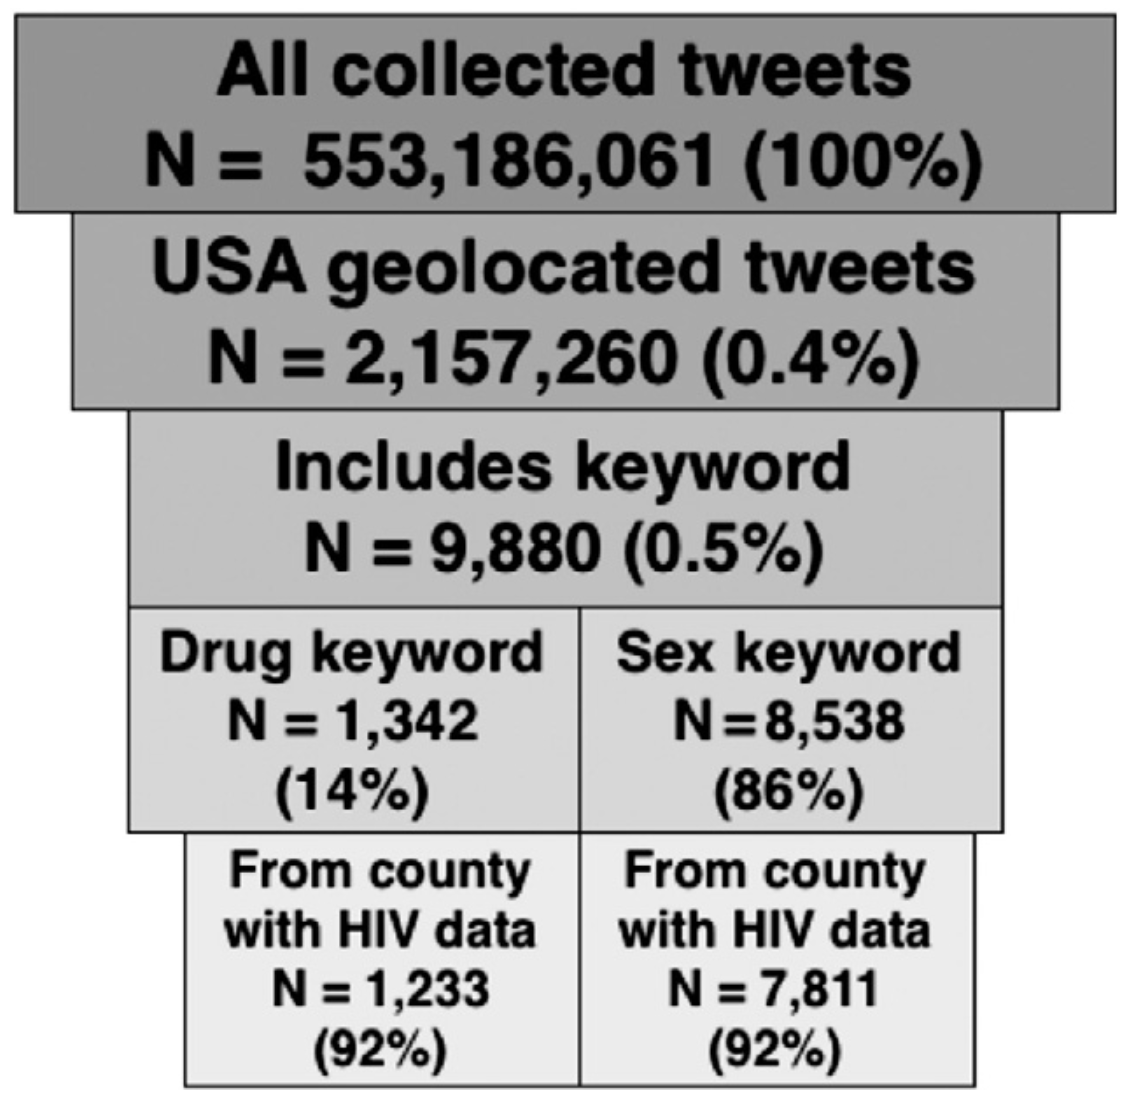
\includegraphics[width=6.5cm]{HIV-Method}
	\caption{Twitter Data Filtering by Young et al \cite{Young:2014aa}.}
	\label{fig:HIV-Method}
\end{figure}

The framework in Figurre \ref{fig:HIV-Method} is one of the bases of this research \cite{Young:2014aa}. From the collection of posts gathered, these data is then validated using aggregated public data that may come  from the Department of Health. Through doing so, a correlation shall be identified to be used as a basis for the predictive model of the diseases.

\textbf{B. Dengue} - In the study made on Dengue surveillance in Brazil, four (4) parameters were used to filter social media posts, particularly tweets. These are \textit{volume}, \textit{location}, \textit{time}, and \textit{public perception} \cite{gomide2011dengue}. The same parameters are taken into consideration for the research on Measles, Influenza, and Typhoid Fever. Added to this, the research proposed five (5) taxonomies [Personal experience, Sarcastic tweets, Opinions, Resource, Marketing] to group the posts according to their sentiments  \cite{gomide2011dengue}. For this research, sentiments are partially disregarded as this may yield to few tweets from Filipinos. If the need for sentiment analysis arises, it may be just to disregard sarcastic tweets, as mentioned in Gomide's research.

\textbf{C. A[H1N1]} - A study on how US-based social media users reacted to the A[H1N1] epidemic was also made to produce an infodemiological surveillance report \cite{Signorini:2011aa}.. Besides the initial filters using the words \textit{``swine"}, \textit{``influenza"}, and \textit{``ah1n1"}, he also utilized a second filtering for other possible related keywords caused by the evolution of public concern. It shows a kind of filtering from specific to general, rather than general to specific. Some example search keywords include vaccines, flight details (to track movement), and even pork products, such as \textit{``bacon"} \cite{Signorini:2011aa}.